
\begin{figure}
	\begin{center}
		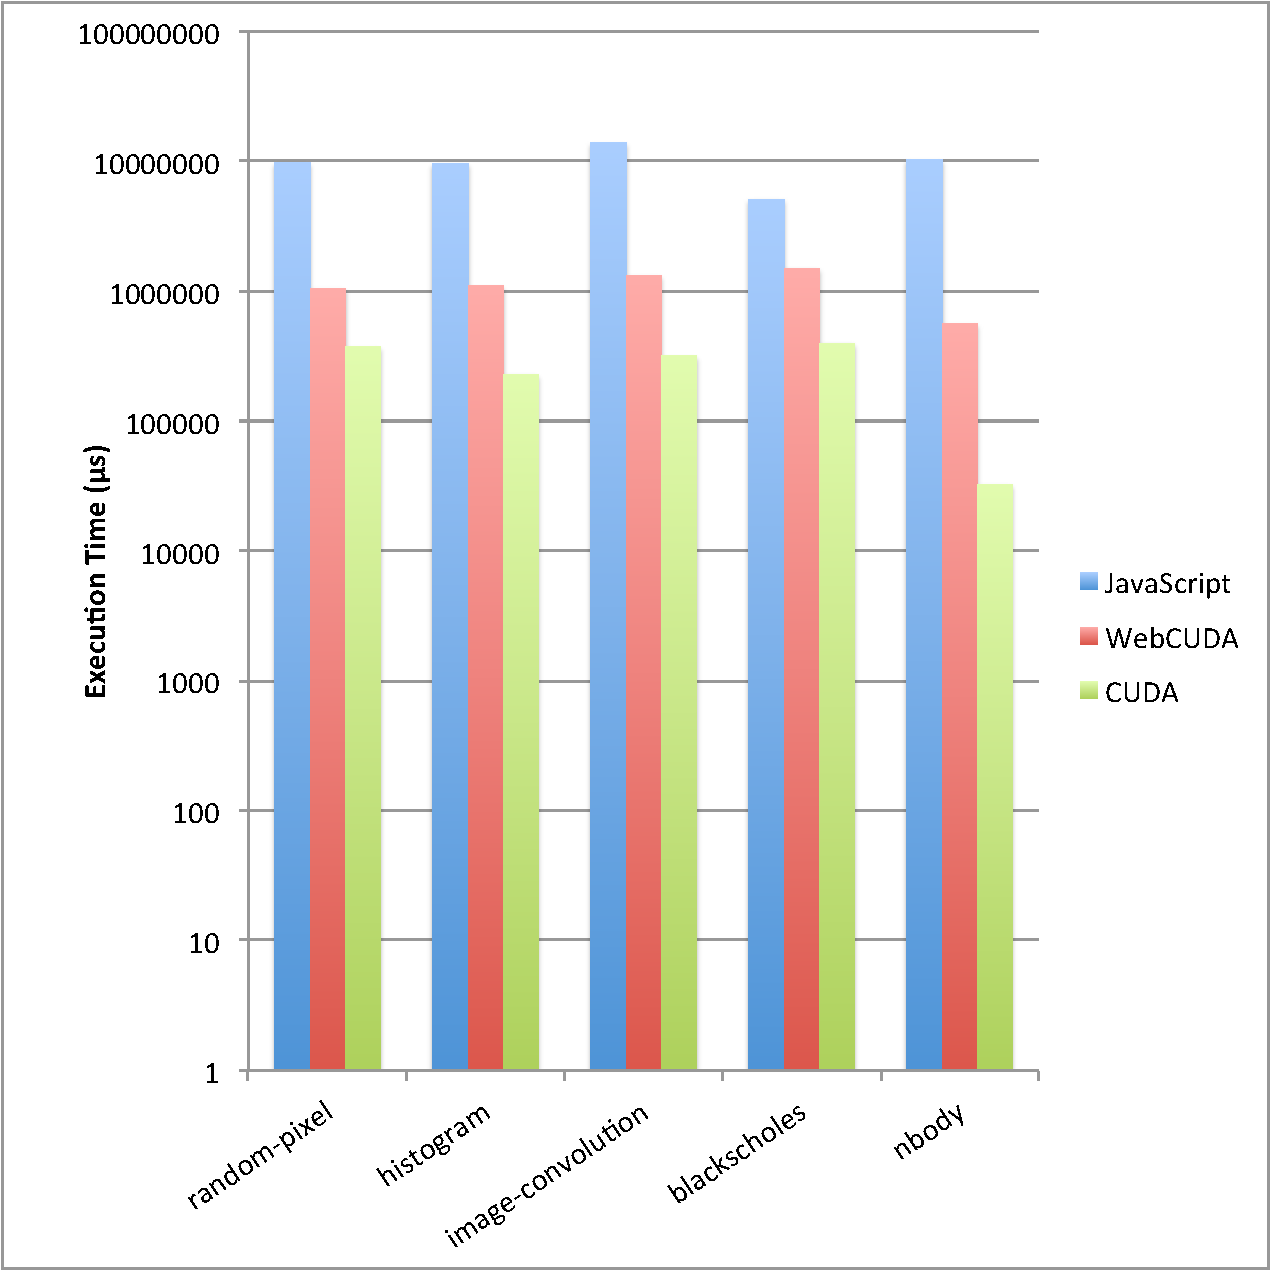
\includegraphics[width=\columnwidth]{./figures/fig1}
	\end{center}
	\caption{Comparison of Execution Time between JavaScript, \namens, and CUDA benchmarks}
	\label{fig1}
\end{figure}

\begin{figure}
	\begin{center}
		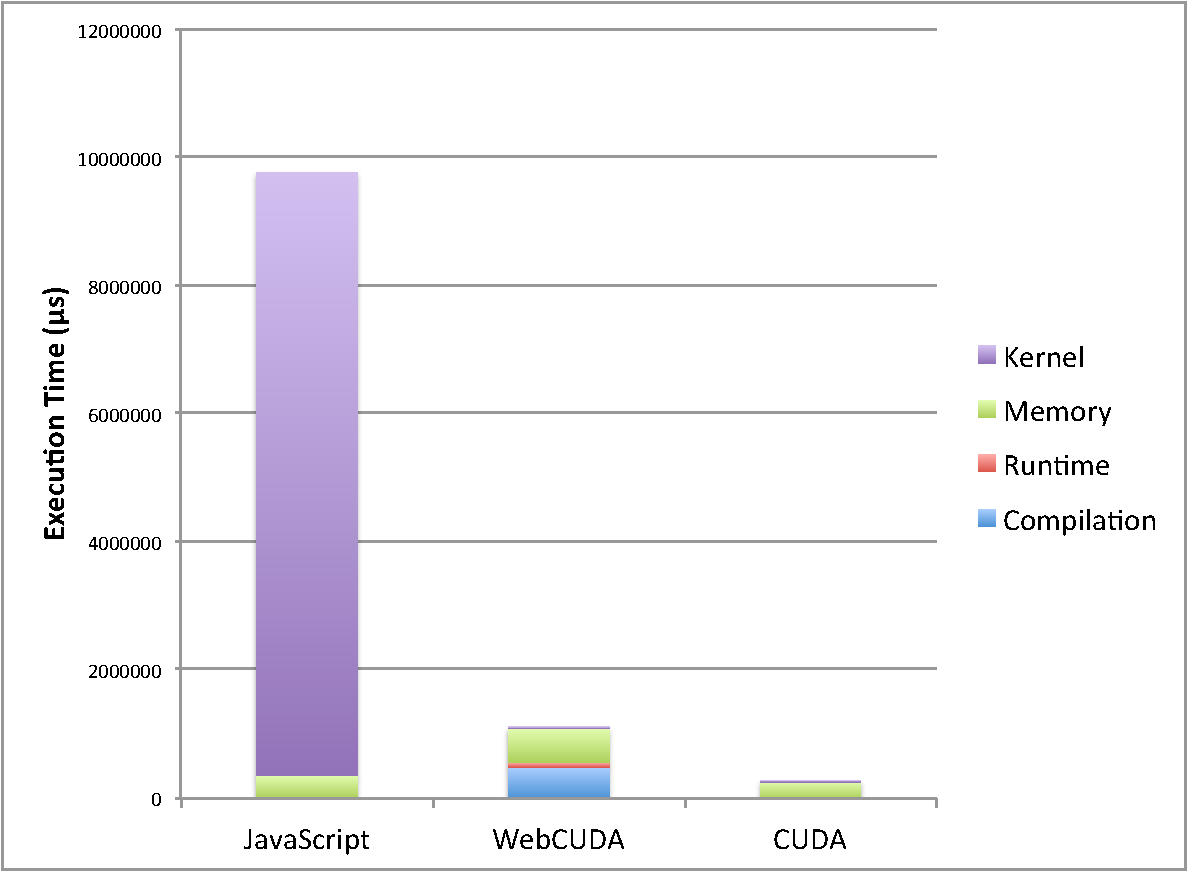
\includegraphics[width=\columnwidth]{./figures/fig2}
	\end{center}
	\caption{Breakdown of Stages of Execution}
	\label{fig2}
\end{figure}

\begin{figure}
	\begin{center}
		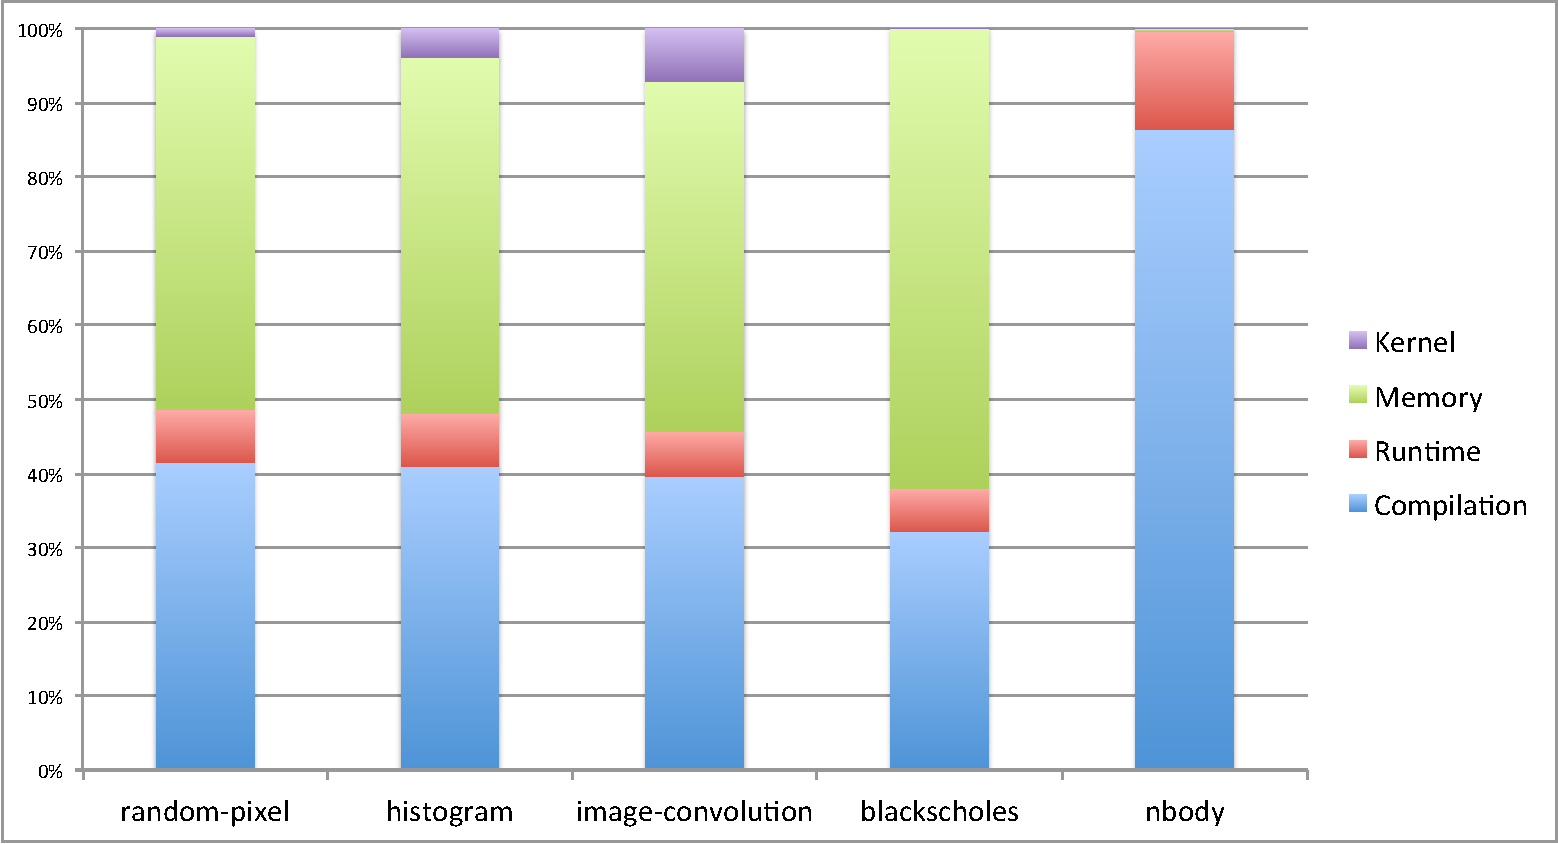
\includegraphics[width=\columnwidth]{./figures/fig3}
	\end{center}
	\caption{Breakdown of Stage of Execution for each \name Benchmark}
	\label{fig3}
\end{figure}

\begin{figure}
	\begin{center}
		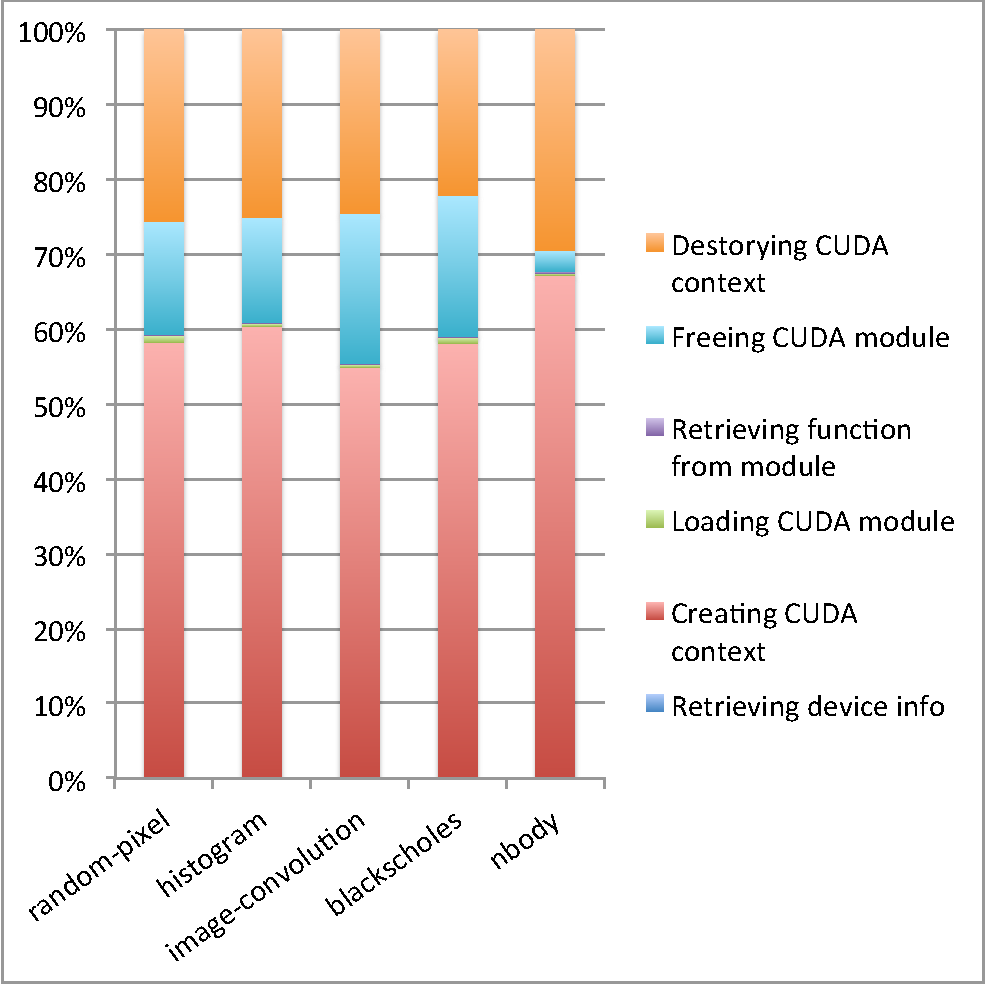
\includegraphics[width=\columnwidth]{./figures/fig4}
	\end{center}
	\caption{Breakdown of Runtime Overhead of \namens}
	\label{fig4}
\end{figure}

We evaluate our WebCUDA implementation with the original V8 JavaScript engine, which servers as a baseline, and the CUDA framework, which is set as a reference.

\subsection{Benchmarks}
\begin{table}
	\begin{center}
		\begin{tabular}{| l | l |}
			\hline
			Benchname & Input/Output Size \\
			\hline
			random-pixel & 32M pixel image \\
			\hline
			histogram & 512M elements \\
			\hline
			image-convolution & 16M pixel image \\
			\hline
			blackscholes & 40M options \\
			\hline
			nbody-simulation & 1024 bodies \\
			\hline
		\end{tabular}
	\end{center}
	\caption{Description of Benchmarks use for evaluation.}
	\label{benchmark-table}
\end{table}

To evaluate performance on different platforms, we create different versions of benchmarks for each platform. We choose 5 CUDA examples provided with corresponding CPU version mostly from CUDA SDK samples, and manually port them to WebCUDA and JavaScript environments. Porting to WebCUDA versions starts from CUDA versions, and involves rewriting CPU portions in JavaScript with WebCUDA extension and wrapping CUDA portions separately as string. Porting to JavaScript versions is more
straightforward, and involves translating C code into JavaScript code line by line.
The input sizes are adjusted as shown in Table 2 to make the amount of computation and the execution time of JavaScript versions nontrivial.

\subsection{Experimental Setup}
We run all experiments on the Amazon EC2 instance to ensure an isolated execution environment. It has Intel Xeon 8-core processor running at 2.6 GHz and NVIDIA GRID K520 based on the Kepler architecture. The CUDA driver and runtime version is set to 5.5 which was the most recent version when the project was started. We build our WebCUDA-enabled JavaScript V8 shell on the instance to execute JavaScript and WebCUDA benchmarks, and we build CUDA benchmarks using NVIDIA CUDA Compiler.

\subsection{Results}

\paragraph{Comparison with JavaScript}
Figure 4 shows that WebCUDA is about an order of magnitude faster than JavaScript, and on average, it achieves 9x speedup over JavaScript. As shown in Figure 5, while JavaScript benchmarks takes most of time on the computation, it is negligible in WebCUDA and CUDA benchmarks thanks to the combination of parallel nature of the benchmarks and CUDA device optimized for such parallel computation. WebCUDA introduces compilation and runtime overhead to make use of CUDA device and some memory overhead
for CUDA memory allocation and data transfer between CPU and CUDA device, but the huge gain from the computation more than justifies such overheads.

\paragraph{Comparison with CUDA}
Compared to CUDA benchmarks, however, WebCUDA still experiences 5x slowdown on average. It is mainly due to two reasons. First, WebCUDA has runtime and compilation overhead which is not present in CUDA. Second, memory allocation on CPU takes much more time on WebCUDA. WebCUDA allocates CPU memory using JavaScript constructor functions while CUDA allocates CPU memory through malloc calls. We suspect that a level of indirection for memory allocation in JavaScript would be a source of
slowdown and leave it as a future work to analyze memory performance between JavaScript and CUDA.

\paragraph{Compilation Overhead}
Figure 6 shows that compilation overhead is significant which takes up 48\% of the total execution time. It is time to translate a cu file, which is a source code written in CUDA, into a ptx file, which is in the form of intermediate representation for the CUDA-enabled graphics driver. WebCUDA provides a mean to load a ptx file or a cubin file instead which will basically remove the compilation overhead and lead to extra 2x speedup over the native JavaScript. A developer may choose to
load a ptx file for better performance at the cost of extra maintenance effort of compiling a cu file offline. In addition, as a ptx file is difficult to read without knowledge of intermediate representation, it will degrade readability and reusability of source code which is one of benefits of web applications.

\paragraph{V8 Runtime Overhead}
Runtime overhead is introduced by WebCUDA Runtime overhead takes 7.9\% on average of the total execution time for WebCUDA benchmarks. As shown in Figure 7, maintaining CUDA execution context is responsible for most of the overhead.

\paragraph{Running Native JavaScript Programs}
To verify that the WebCUDA extension does not negatively affect native JavaScript programs, we run Octane Benchmark Suite on the original V8 and our WebCUDA-enabled V8. Octane Benchmark Suite is a popular JavaScript benchmark suite consisting of 17 programs ranging from traditional scientific benchmarks to realistic web applications, and reports test scores based on the execution time. We ran it multiple times on the original and modified V8 versions, and the test scores were about 20,000
with a marginal noise.
